\chapter{Risultati}

L'intervista è stata inviata a 60 infermieri, di cui 9 non hanno risposto all'invito: in totale sono stati raccolti 51 questionari. I professionisti che hanno aderito allo studio lavorano nei seguenti reparti: 18 in Clinica Pediatrica, 13 nel servizio di Day Hospital Pediatrico, 13 nella struttura di Oncoematologia, 5 in quella di Ortopedia e Traumatologia e 2 in quella di Radiologia Pediatrica - servizio di Risonanza Magnetica. Gli anni di esperienza degli intervistati variano da 6 mesi a 36 anni, con una mediana di 10 anni (IQR\footnote{\emph{Interquartile Range} o lo scarto interquartile: è la differenza tra il terzo ed il primo quartile.} 2-22.75). 27 infermieri (53$\%$) assistono meno di 10 sedazioni procedurali al mese, 14 (27.4$\%$) da 10 a 20, 8 (15.7$\%$) da 21 a 30 e 2 (3.9$\%$) più di 30 sedazioni ogni mese. 

\begin{figure}[h]
    \centering
    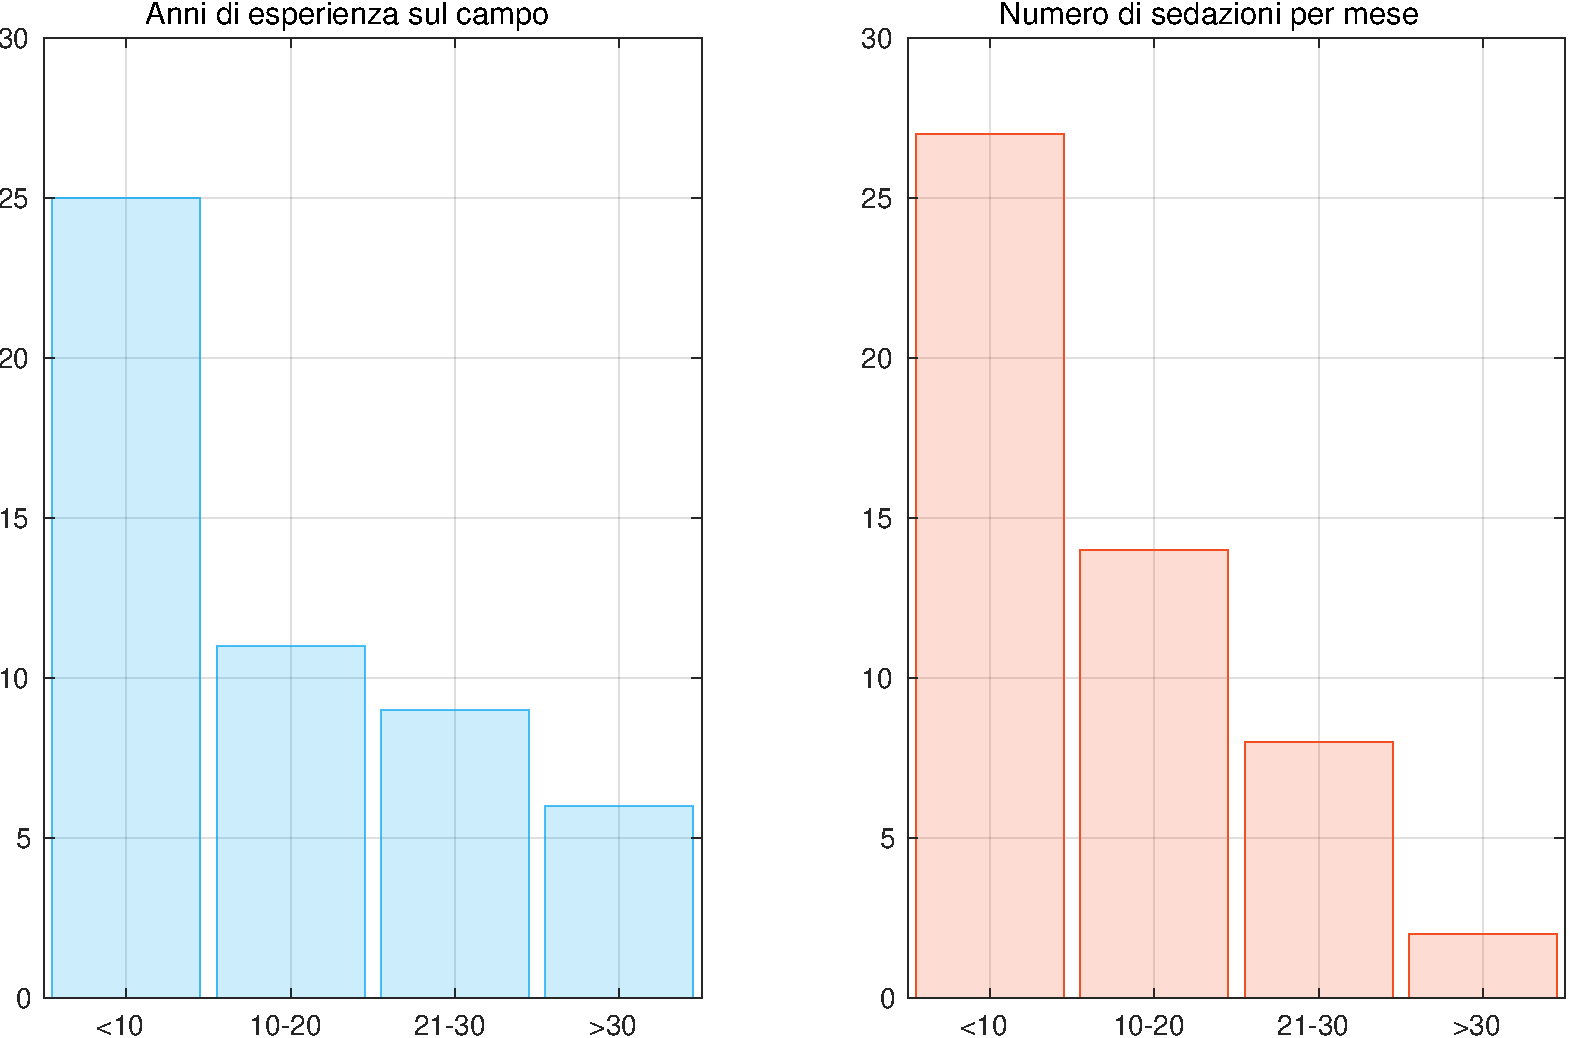
\includegraphics[width=0.7\textwidth]{Figure/esperienzaVSfrequenza.pdf}
    \caption{Anni di esperienza nel campo delle sedazioni procedurali e numero di sedazioni mensilmente assistite.}
    \label{fig:esperienzavsfrequenza}
\end{figure}

\subsection*{Qualità globale della sedazione}
Gli infermieri intervistati hanno dato una valutazione elevata a quasi tutti i farmaci testati: in particolare 32 partecipanti hanno attribuito un punteggio\footnote{Il grado di soddisfazione è stato misurato secondo scala \texttt{NRS}, da 0 a 10.} $\geq$8 alla qualità della sedazione con il propofol, 26 a quella con il midazolam, 23 a quella con la dexmedetomidina. I livelli di soddisfazione più bassi sono stati riscontrati con l'utilizzo della ketamina, infatti solo 8 persone hanno assegnato un punteggio $\geq$8. Nella figura \ref{fig:qualitascolorful} si possono osservare i valori della mediana, del primo e del terzo quartile relativi al livello di soddisfazione percepito dal personale infermieristico, riportati anche numericamente nella tabella \ref{tab:qualitased}: si evince una differenza statisticamente significativa tra le mediane dei punteggi per i differenti farmaci sedativi ed analgesici (Kruskal-Wallis p-value 0.005), in particolare la ketamina ha mostrato un valore significativamente inferiore rispetto al propofol (p-value Bonferroni <0.001), al midazolam (p-value Bonferroni 0.005) ed alla dexmedetomidina (p-value Bonferroni 0.003).

\begin{figure}[h]
    \centering
    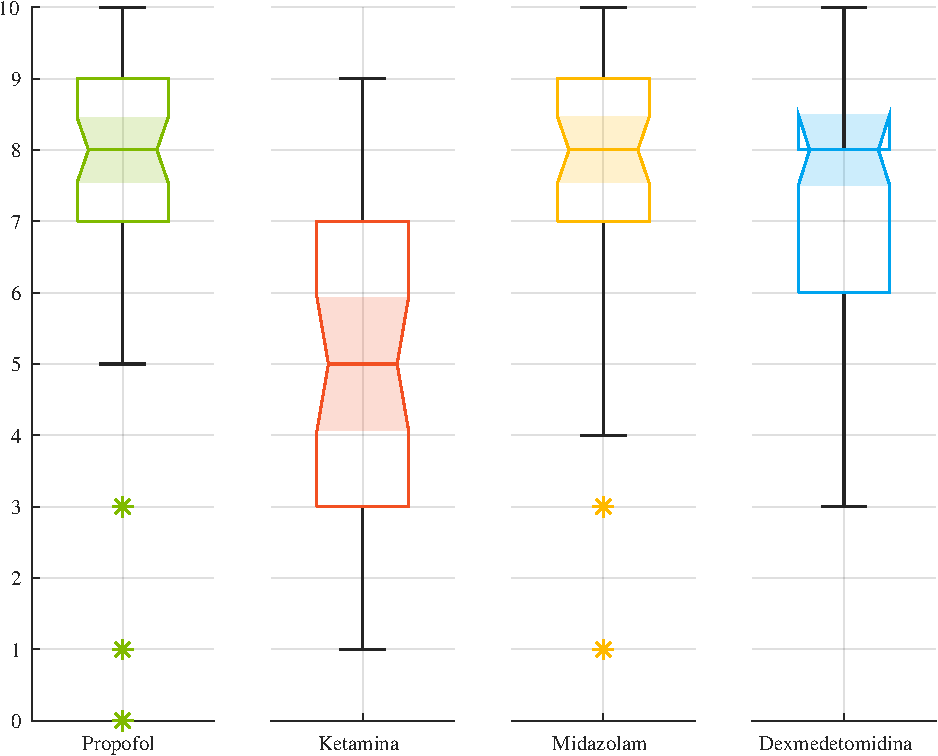
\includegraphics[width=0.8\textwidth]{Figure/qualita-colorful.pdf}
    \caption{Confronto del livello di soddisfazione percepito dagli infermieri (misurato in scala \texttt{NRS}) in relazione ai quattro agenti farmacologici testati in questo lavoro di tesi.}
    \label{fig:qualitascolorful}
\end{figure}

\bgroup
\def\arraystretch{1.5}
\begin{table}[h]
    \centering
    \begin{tabular}{|l|l|}
         Regimi farmacologici & Mediana (IQR) \\ \hline
       Propofol & 8 (7-9)  \\
       Ketamina & 5 (3-7) \\
       Midazolam & 8 (7-9) \\
       Dexmedetomidina & 8 (6-8) 
    \end{tabular}
    \caption{Valori di mediana e quartili associati alla qualità complessiva della sedazione con i quattro agenti farmacologici.}
    \label{tab:qualitased}
\end{table}
\egroup

%\subsection*{Elementi che influenzano il grado di soddisfazione}

\subsection*{Grado di sicurezza percepito ed effetti avversi}

Il livello di sicurezza percepito durante la sedazione è risultato elevato per tutti i farmaci usati, senza alcuna differenza statisticamente significativa (Kruskal-Wallis p-value 0.08). I risultati sono rappresentati nella figura e i valori di mediana e IQR descritti nella tabella\footnote{I dati numerici sono ottenuti attribuendo un valore pari ad 1 alla risposta \emph{per niente}, pari a 6 per \emph{poco}, pari a 10 per \emph{molto}.}.

\begin{figure}[!h]
    \centering
    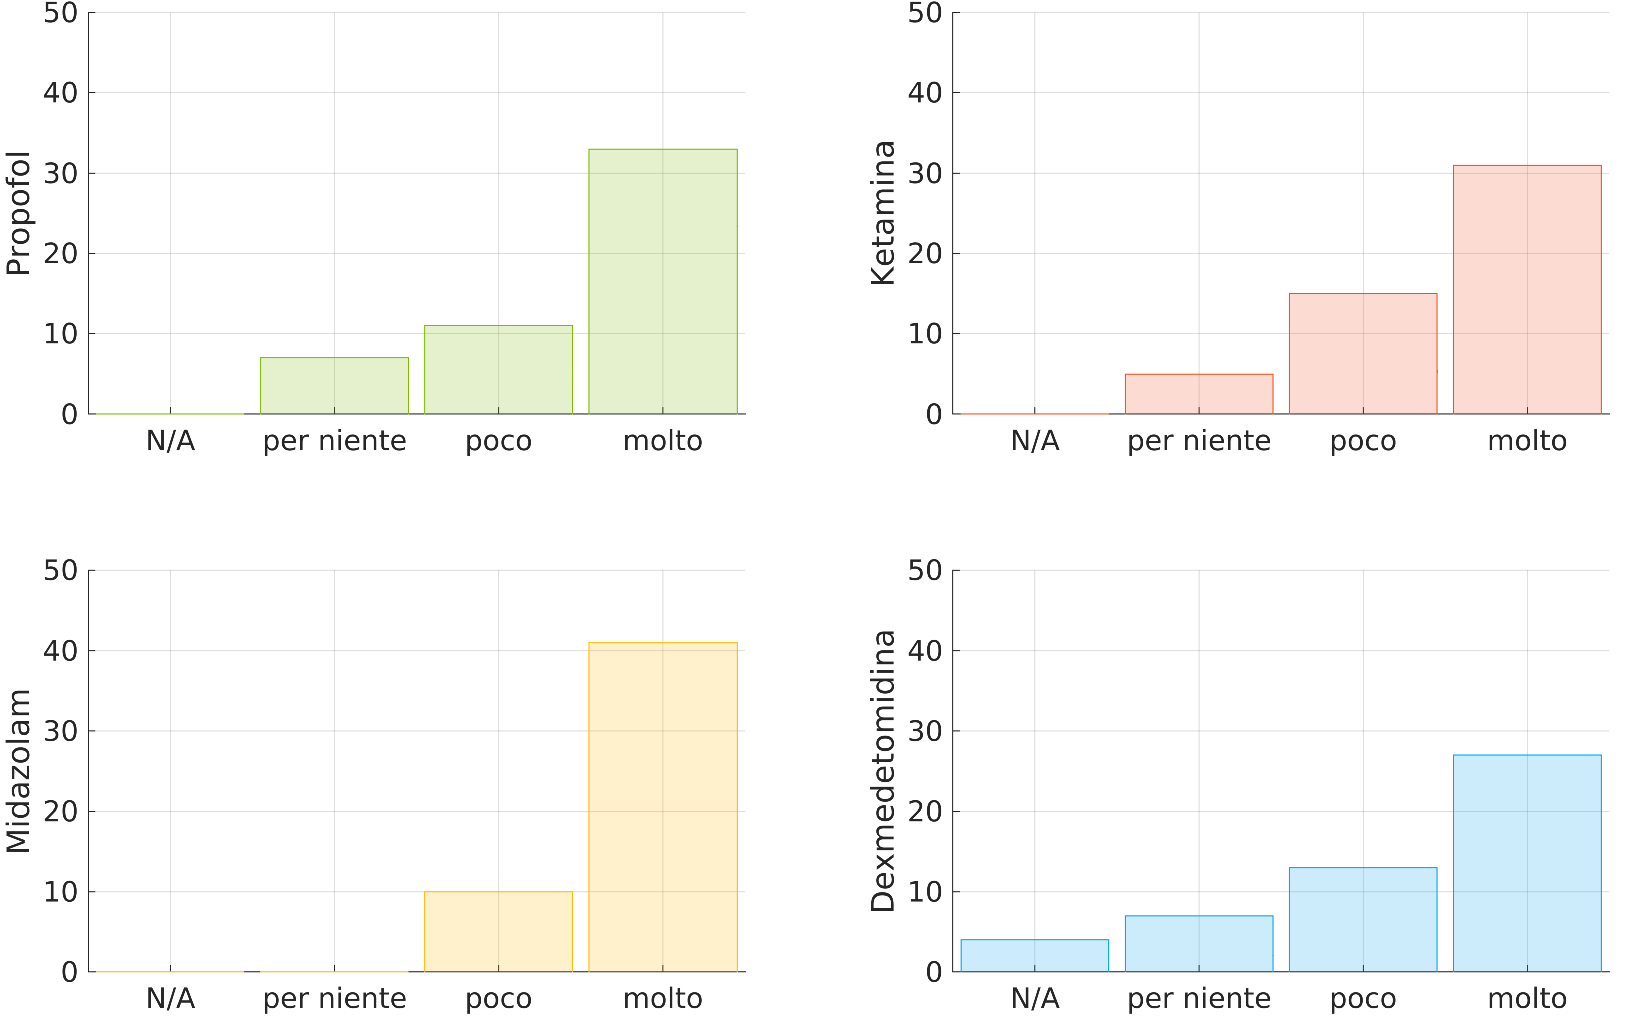
\includegraphics[width=0.9\textwidth]{Figure/sicurezza.pdf}
    \caption{Le risposte del personale infermieristico alla domanda "Quanto ti senti sicuro durante la sedazione con i seguenti farmaci?"}
    \label{fig:sicurezza}
\end{figure}

\bgroup
\def\arraystretch{1.5}
\begin{table}[h]
    \centering
    \begin{tabular}{|l|l|}
         Regimi farmacologici & Mediana (IQR) \\ \hline
       Propofol & 8 (7-9)  \\
       Ketamina & 8 (6-9) \\
       Midazolam & 9 (7-9.5) \\
       Dexmedetomidina & 7.5 (4-8) 
    \end{tabular}
    \caption{Valori di mediana e quartili associati alla sicurezza percepita durante la sedazione con i quattro agenti farmacologici.}
    \label{tab:sicurezzased}
\end{table}
\egroup

\subsection*{Correlazione lineare tra esperienza e preferenze farmacologiche}

Stratificando il grado di soddisfazione percepito dal personale infermieristico con gli anni di esperienza compiuti nel campo delle sedazioni procedurali o con il numero di sedazioni mensilmente effettuate non risultano differenze statisticamente significative, come graficamente visibile nelle figure \ref{fig:qualitaesperienza}, \ref {fig:qualitafrequenza}.

\begin{figure}[h]
    \centering
    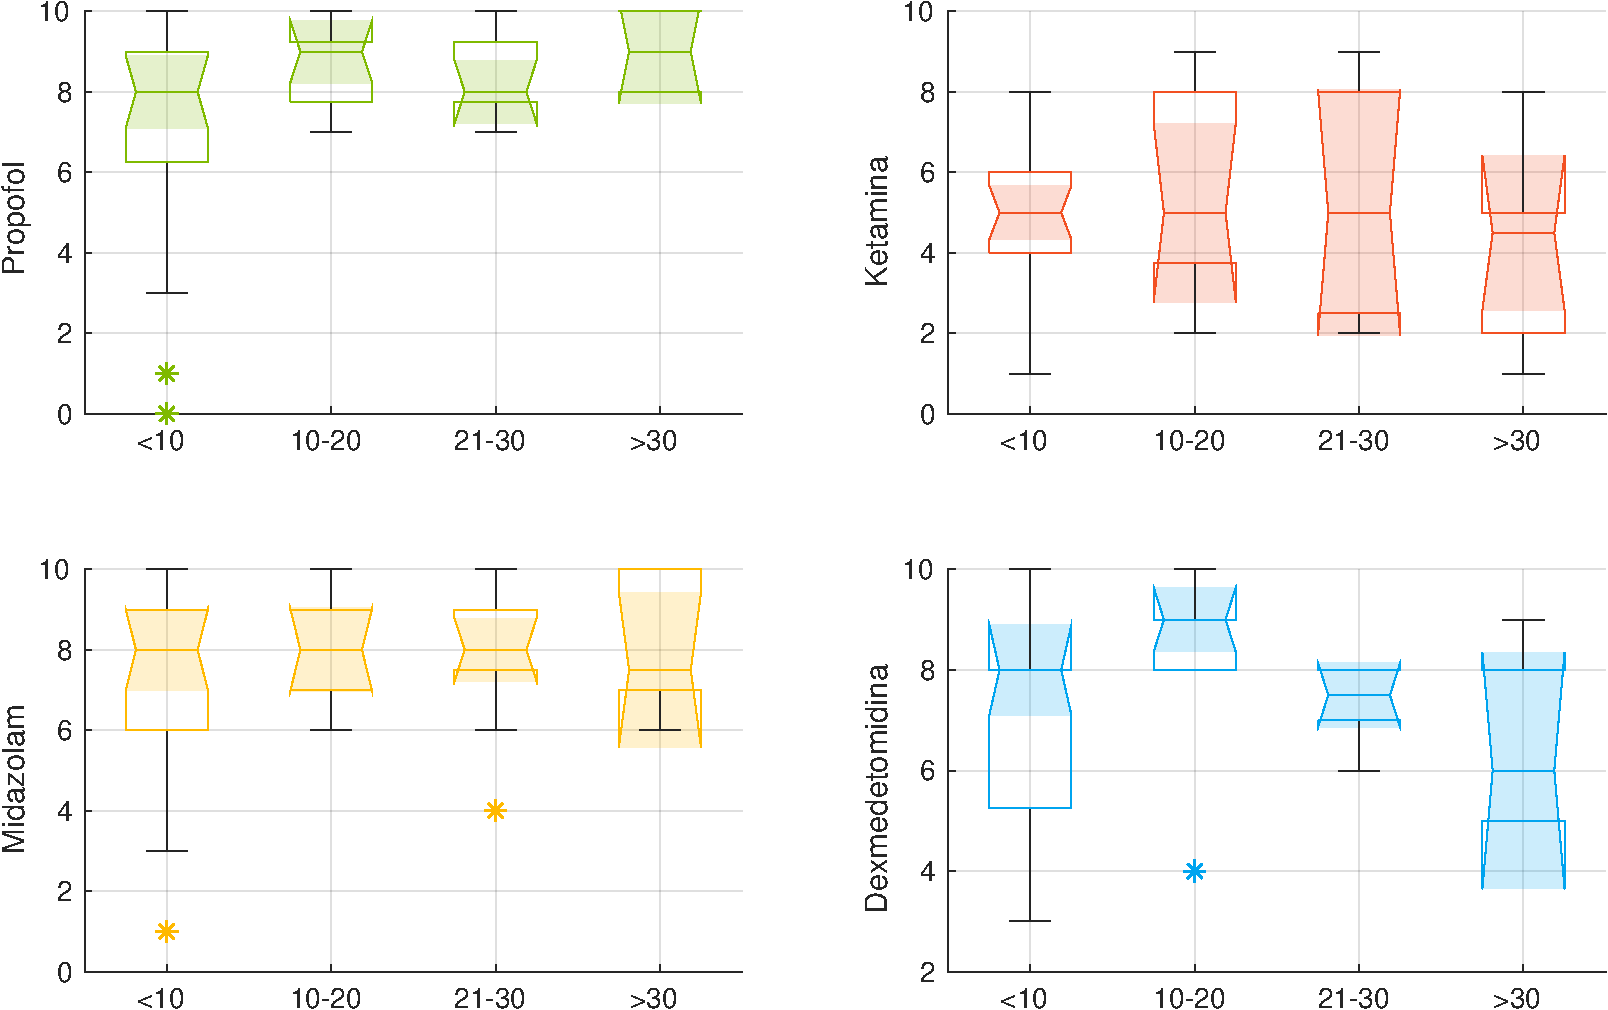
\includegraphics[width=0.65\textwidth]{Figure/qualita-strat-esperienza.pdf}
    \caption{Livello di soddisfazione associato ai diversi agenti farmacologici (misurato secondo scala NRS) stratificato per gli anni di esperienza dei partecipanti nell'ambito delle sedazioni procedurali.}
    \label{fig:qualitaesperienza}
\end{figure}

\begin{figure}[!h]
    \centering
    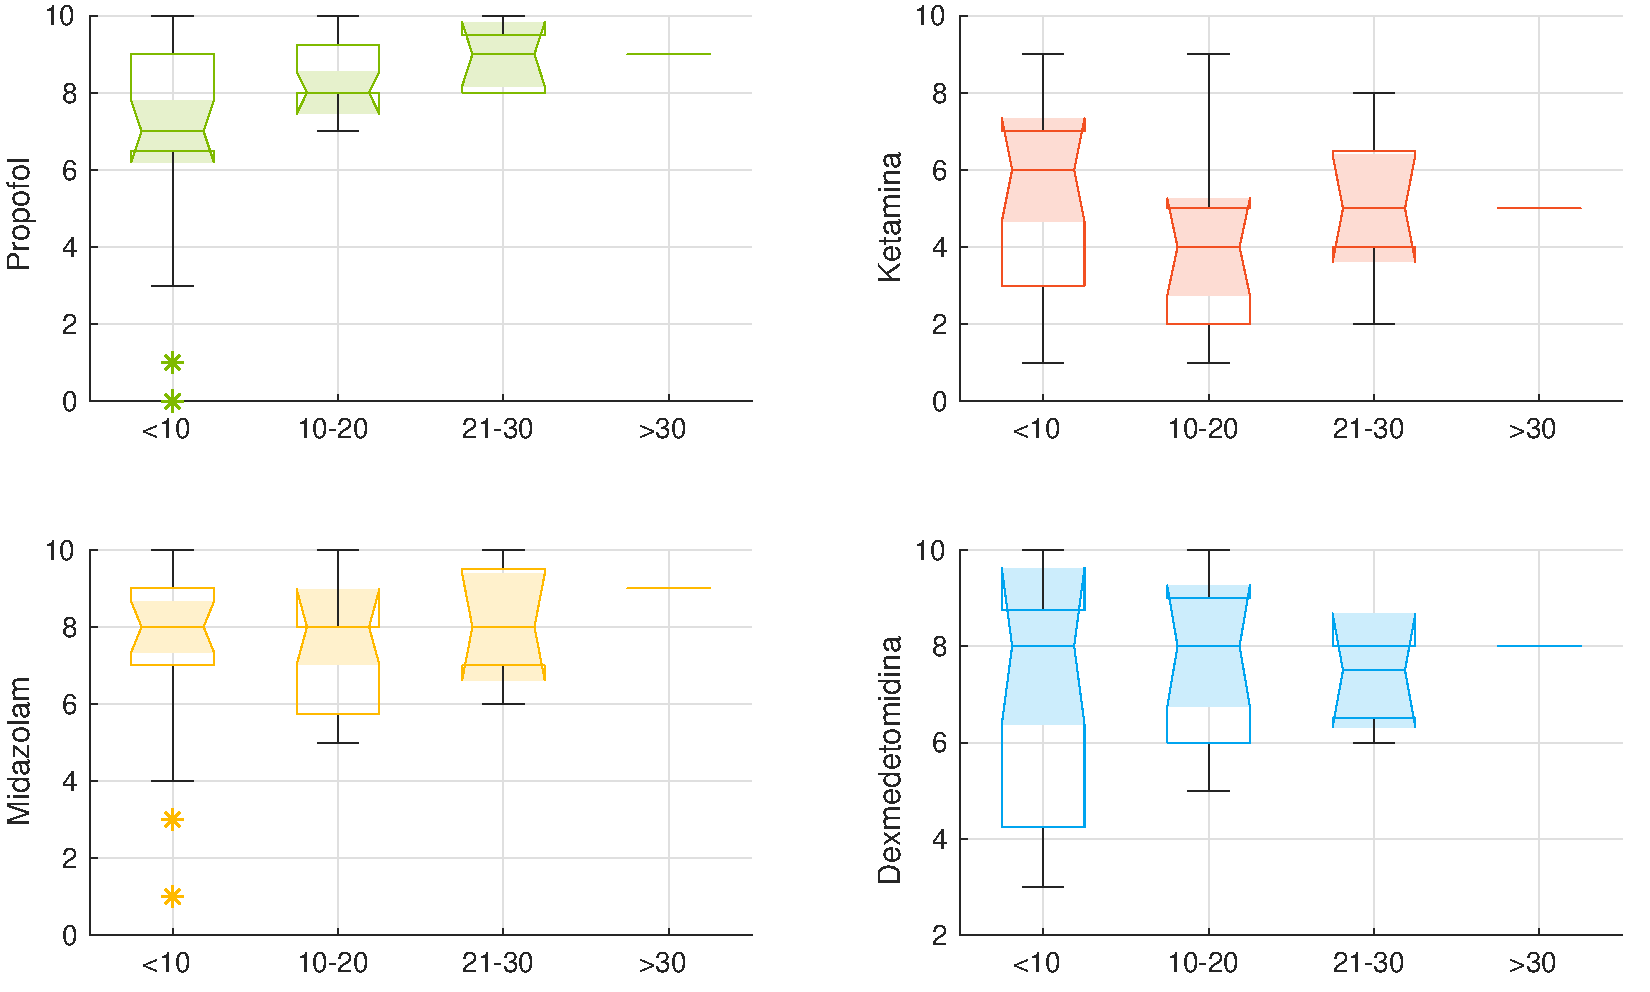
\includegraphics[width=0.65\textwidth]{Figure/qualita-strat-frequenza.pdf}
    \caption{Livello di soddisfazione associato ai diversi agenti farmacologici (misurato secondo scala NRS) stratificato per il numero di sedazioni mensilmente assistite dagli intervistati.}
    \label{fig:qualitafrequenza}
\end{figure}

\subsection*{Preferenze relative alle vie di somministrazione}

Le vie di somministrazione preferite dagli infermieri sono, in ordine di preferenza: via endovenosa (scelta da 28 persone - 55$\%$), via orale più intranasale (15 - 29.5$\%$), via intranasale (7 - 13.5$\%$) e via intramuscolare (1 - 2$\%$). 

\begin{figure}[!h]
    \centering
    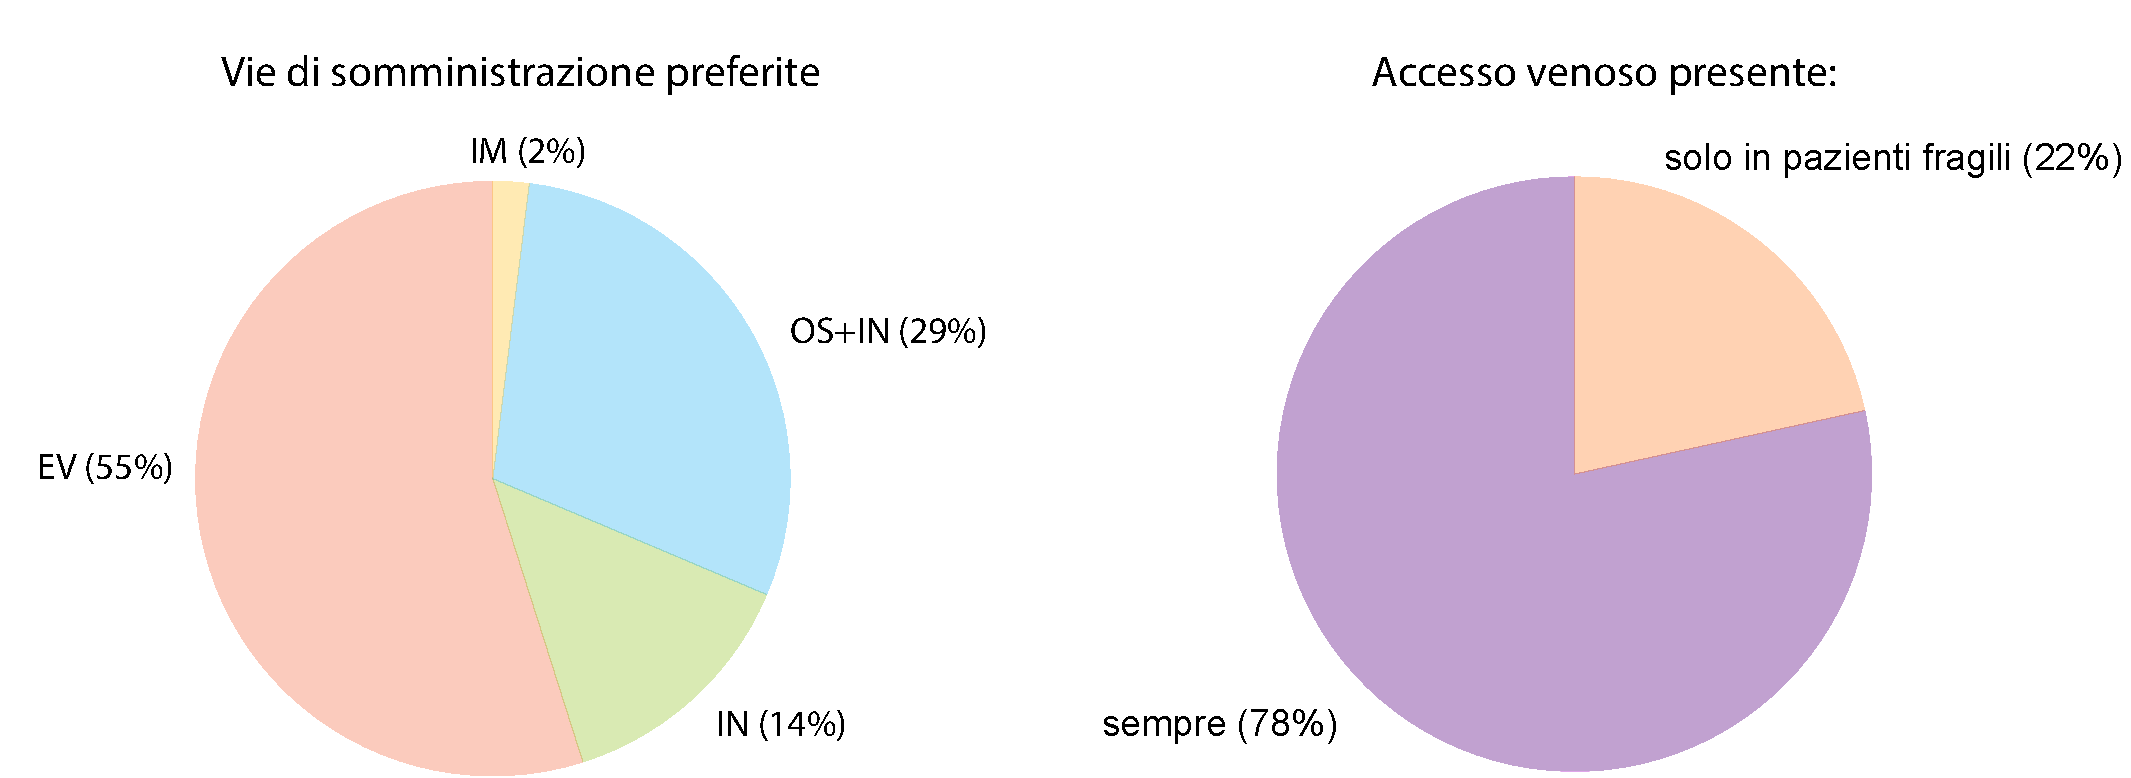
\includegraphics[width=1\textwidth]{Figure/sommicrosoftchiaro.pdf}
    \caption{Vie di somministrazione più apprezzate dagli infermieri per la sedazione procedurale e preferenze relative alla presenza o meno dell'accesso venoso.}
    \label{fig:viedisomm}
\end{figure}



%\subsection*{L'importanza dell'approccio non farmacologico}

